% !TEX root = ../thesis.tex
\chapter{Project Research}
\label{chap:research}
We've previously seen that ``Tone \& Sculpt'' is an existing similar application
on the market. Below we'll consider other background research on existing
systems and their functionality.

The bulk of fitness mobile applications fall into 2 categories:
\begin{enumerate}
	\item Applications which allow fitness enthusiasts to monitor their training
	      and nutrition - the market leaders in this space
	      (by monthly active users) are ``Fitbit''
	      and ``My Fitness Pal'' (as of March 2018) \cite{statista-monthly-users}.
	\item Applications which allow trainers to facilitate the delivery of programmes
	      either by partnering with the development company or white labelling software.
	      These are apps focused on trainers more than end users - the most notable player
	      in this emerging market would be ``TrueCoach''\href{https://truecoach.co/} , who
	      raised USD 2.6 million in seed round funding before being
	      acquired by TSG (Transaction Services Group) in April 2020 \cite{truecoach-funding}.
	      Estimated revenue over USD 1.2 million (from 20k users) for 2021 \cite{truecoach-revenue}.
\end{enumerate}

We can see the main difference in these groups are that
the focus of the former is B2C (business-to-consumer) services
whereas the latter focus on B2B (business-to-business; often acting as SaaS companies).
This is an important distinction as \textit{the project} is looking to combine elements
of both and so the following research will reflect this.
\par
We'll also look at vertical jump calculators and the mathematics involved in developing
something of that nature.
\pagebreak

\section{Existing fitness application systems}
We'll look at 4 systems, 2 from each of the aforementioned application groups. Here it is
worth mentioning that some apps are on the borderline such as
``Centr by Chris Hemsworth''\href{https://centr.com/}. The app follows a B2C approach
but is marketed and part-owned by Chris Hemsworth, with his trainers being the facilitators of programmes
and nutrition plans. A similar approach to the aforementioned
\hyperref[sec:intro_motivation]{``female-focused Tone \& Sculpt''}.
Because cases like these are not relevant to the application being built
for the project, we will not look in any depth at these.
\par
For each of these systems we'll be looking at:
\begin{itemize}
	\item A typical user story for the given application.
	\item A high-level breakdown of the system(s) functionality.
	\item A look at the technology in use (where possible).
\end{itemize}
We'll then compare the applications (in pairs) to see any unique features
and to understand which functions are seemingly core to a positive user experience
in the fitness application space.

\subsection{MyFitnessPal}
\begin{figure}[H]
    \centering
    \begin{minipage}{0.5\textwidth}
        \centering
        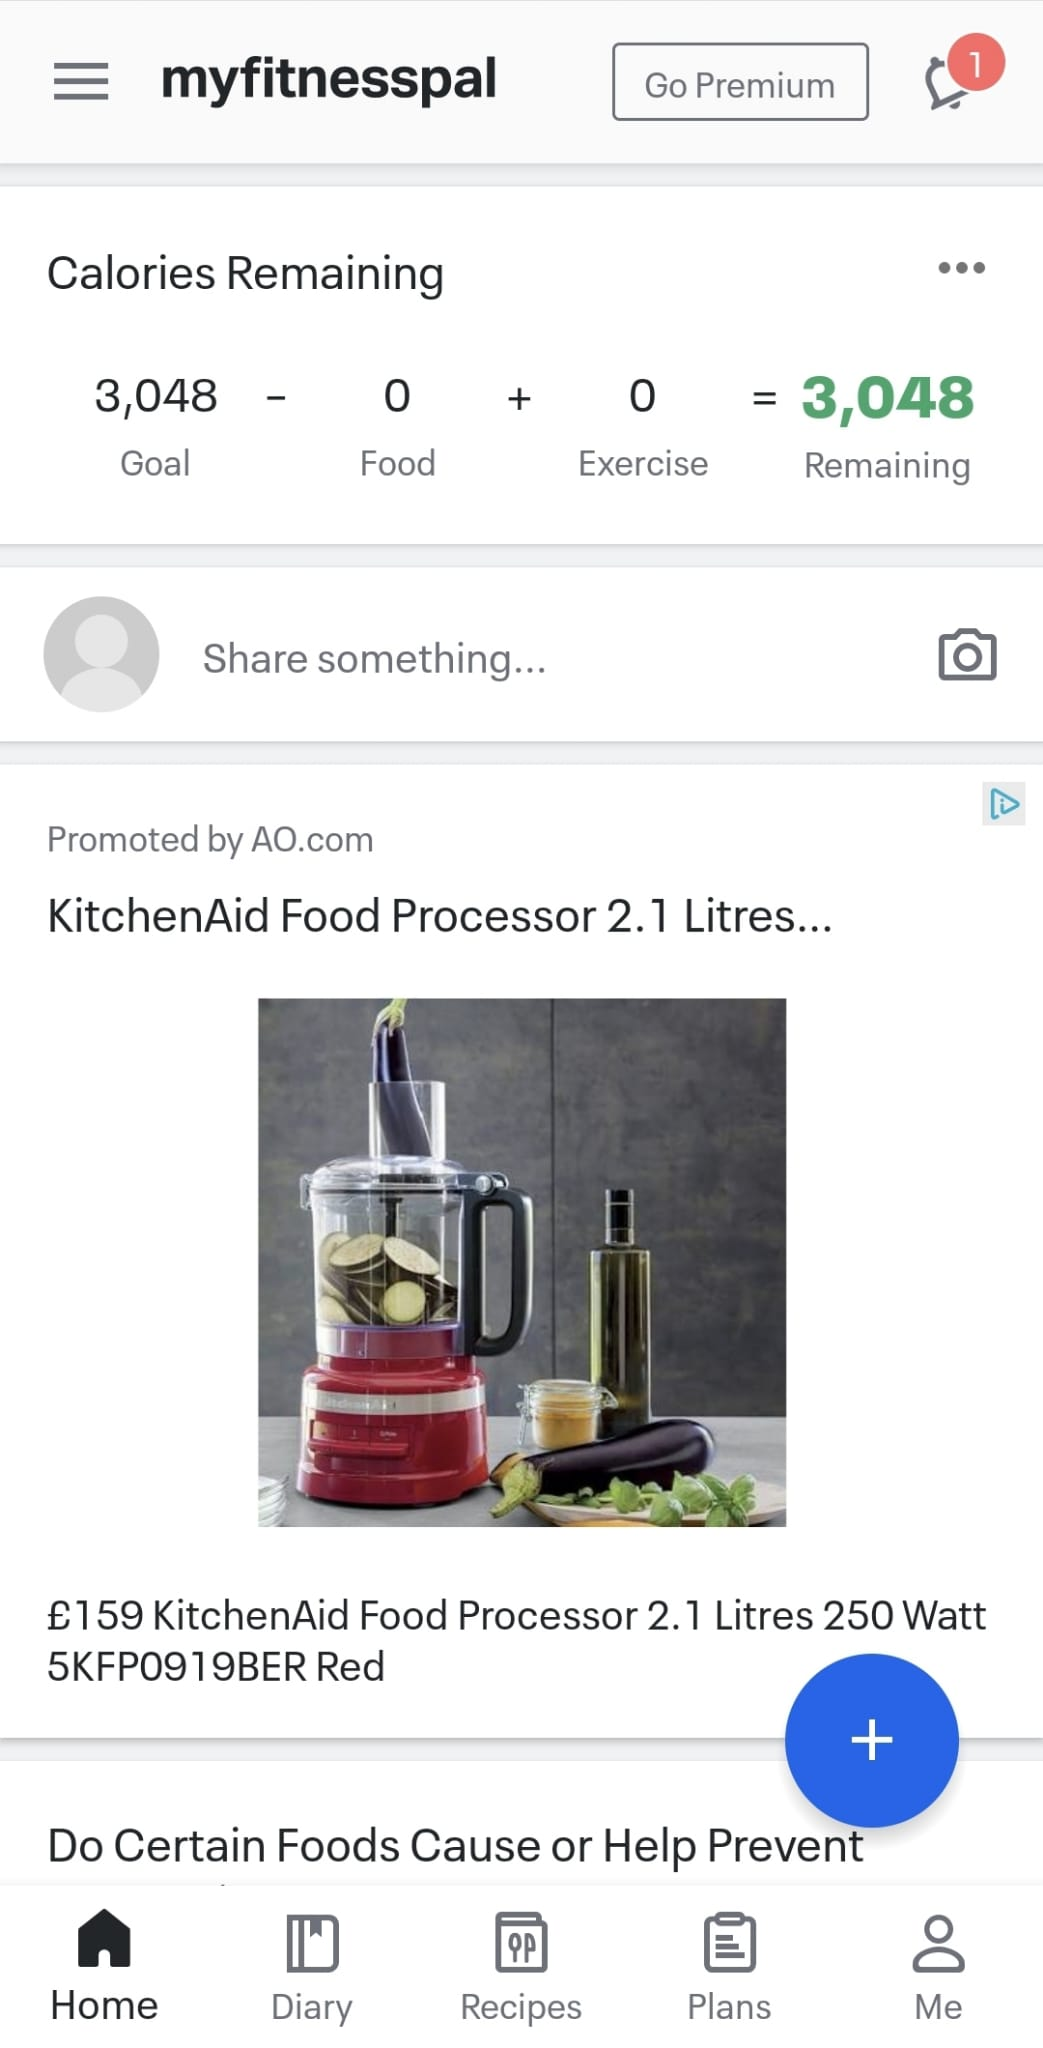
\includegraphics[width=0.5\textwidth]{myfitnesspal/homepage.jpeg}
        \caption{Homepage feed}
        \label{fig:mfp-home}
    \end{minipage}%
    \begin{minipage}{0.5\textwidth}
        \centering
        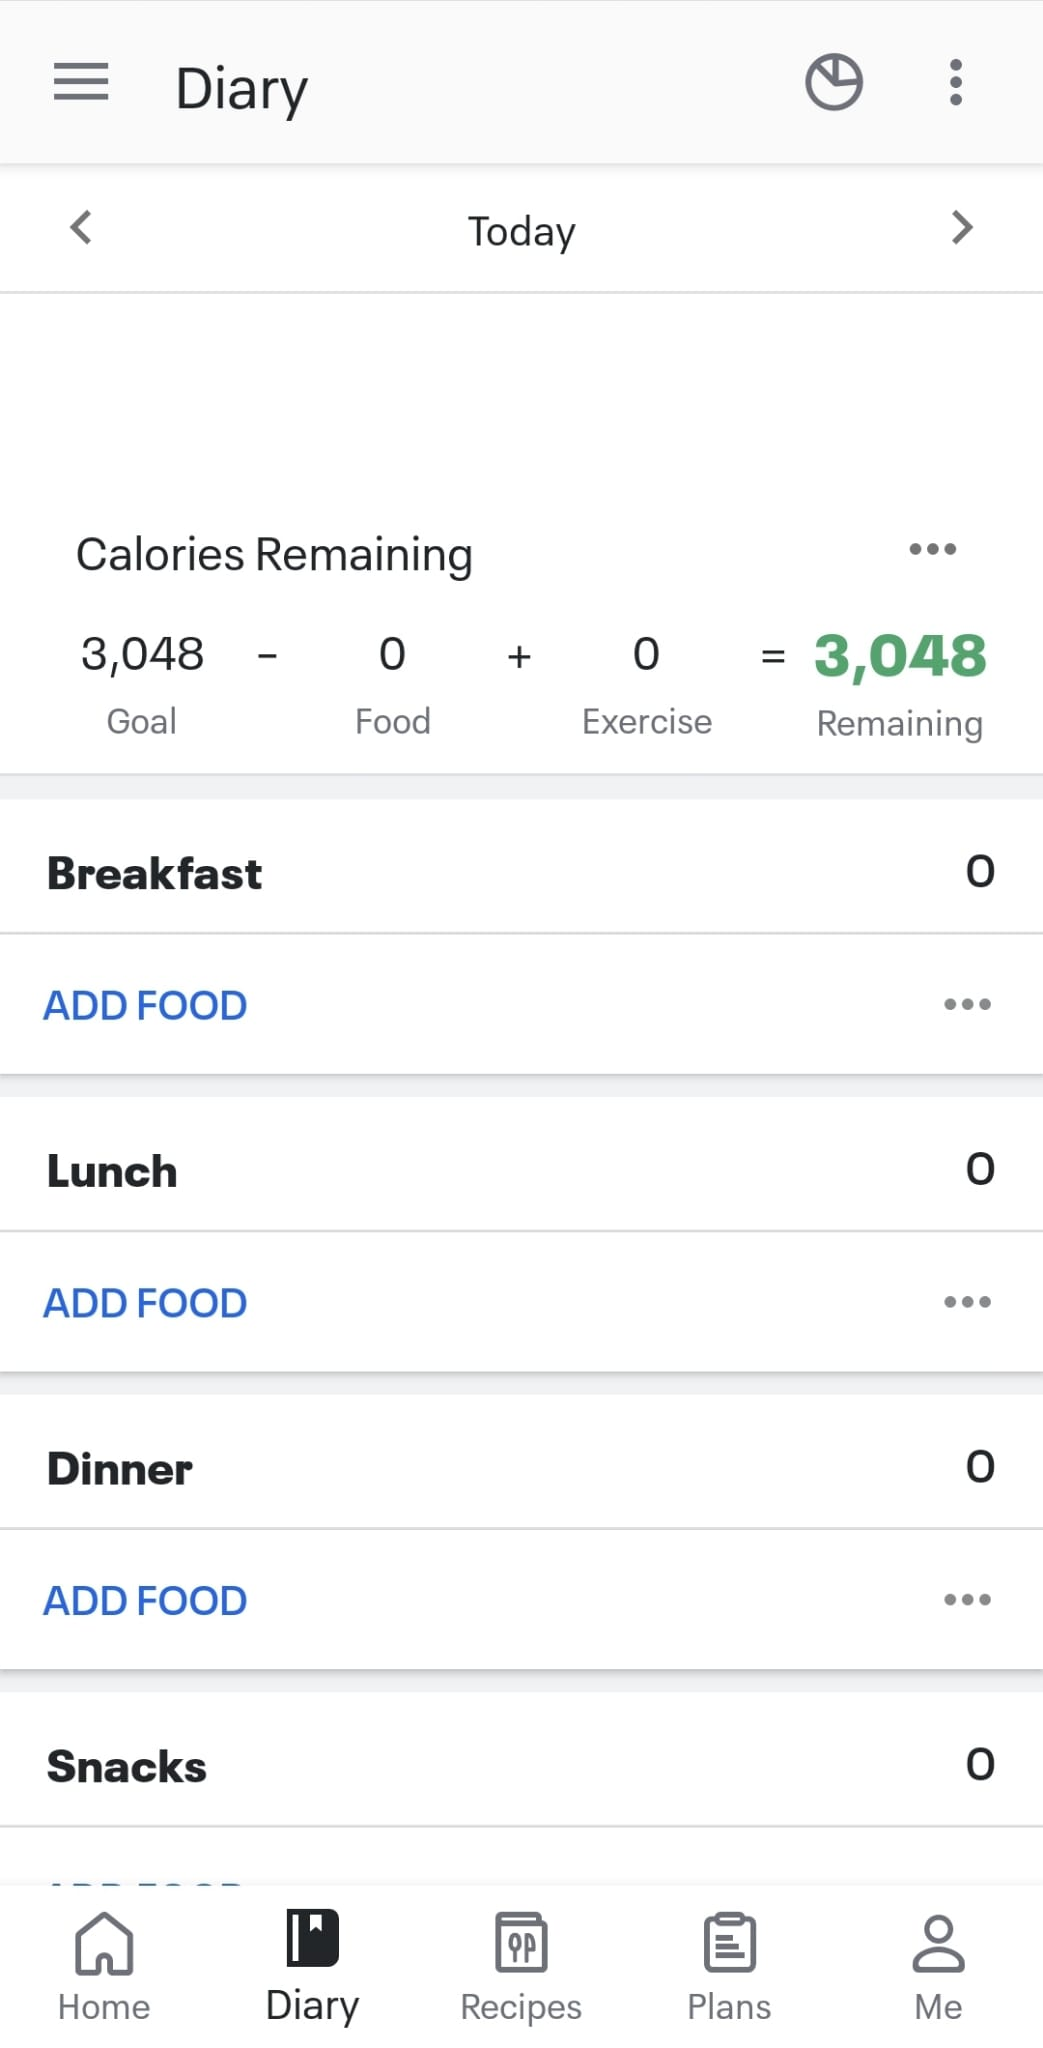
\includegraphics[width=0.5\textwidth]{myfitnesspal/calorie-counter.jpeg}
        \caption{Food diary \& calorie counter}
        \label{fig:mfp-diary}
    \end{minipage}%
\end{figure}
\textbf{User Story}
\label{research-breakdown:mfp-usr-story}
\par
``As a fitness enthusiast, I sign up to the app via email. I wake up
every day and log my breakfast by scanning barcodes for my food.
This is accounted for in my daily food tracking (\cref{fig:mfp-diary}).
After breakfast I create a new workout based on advice from my community or homepage,
I search for the exercises involved and log my workout later on in the day (\cref{fig:mfp-screens}).''
\begin{figure}[H]
    \begin{minipage}{0.5\textwidth}
        \centering
        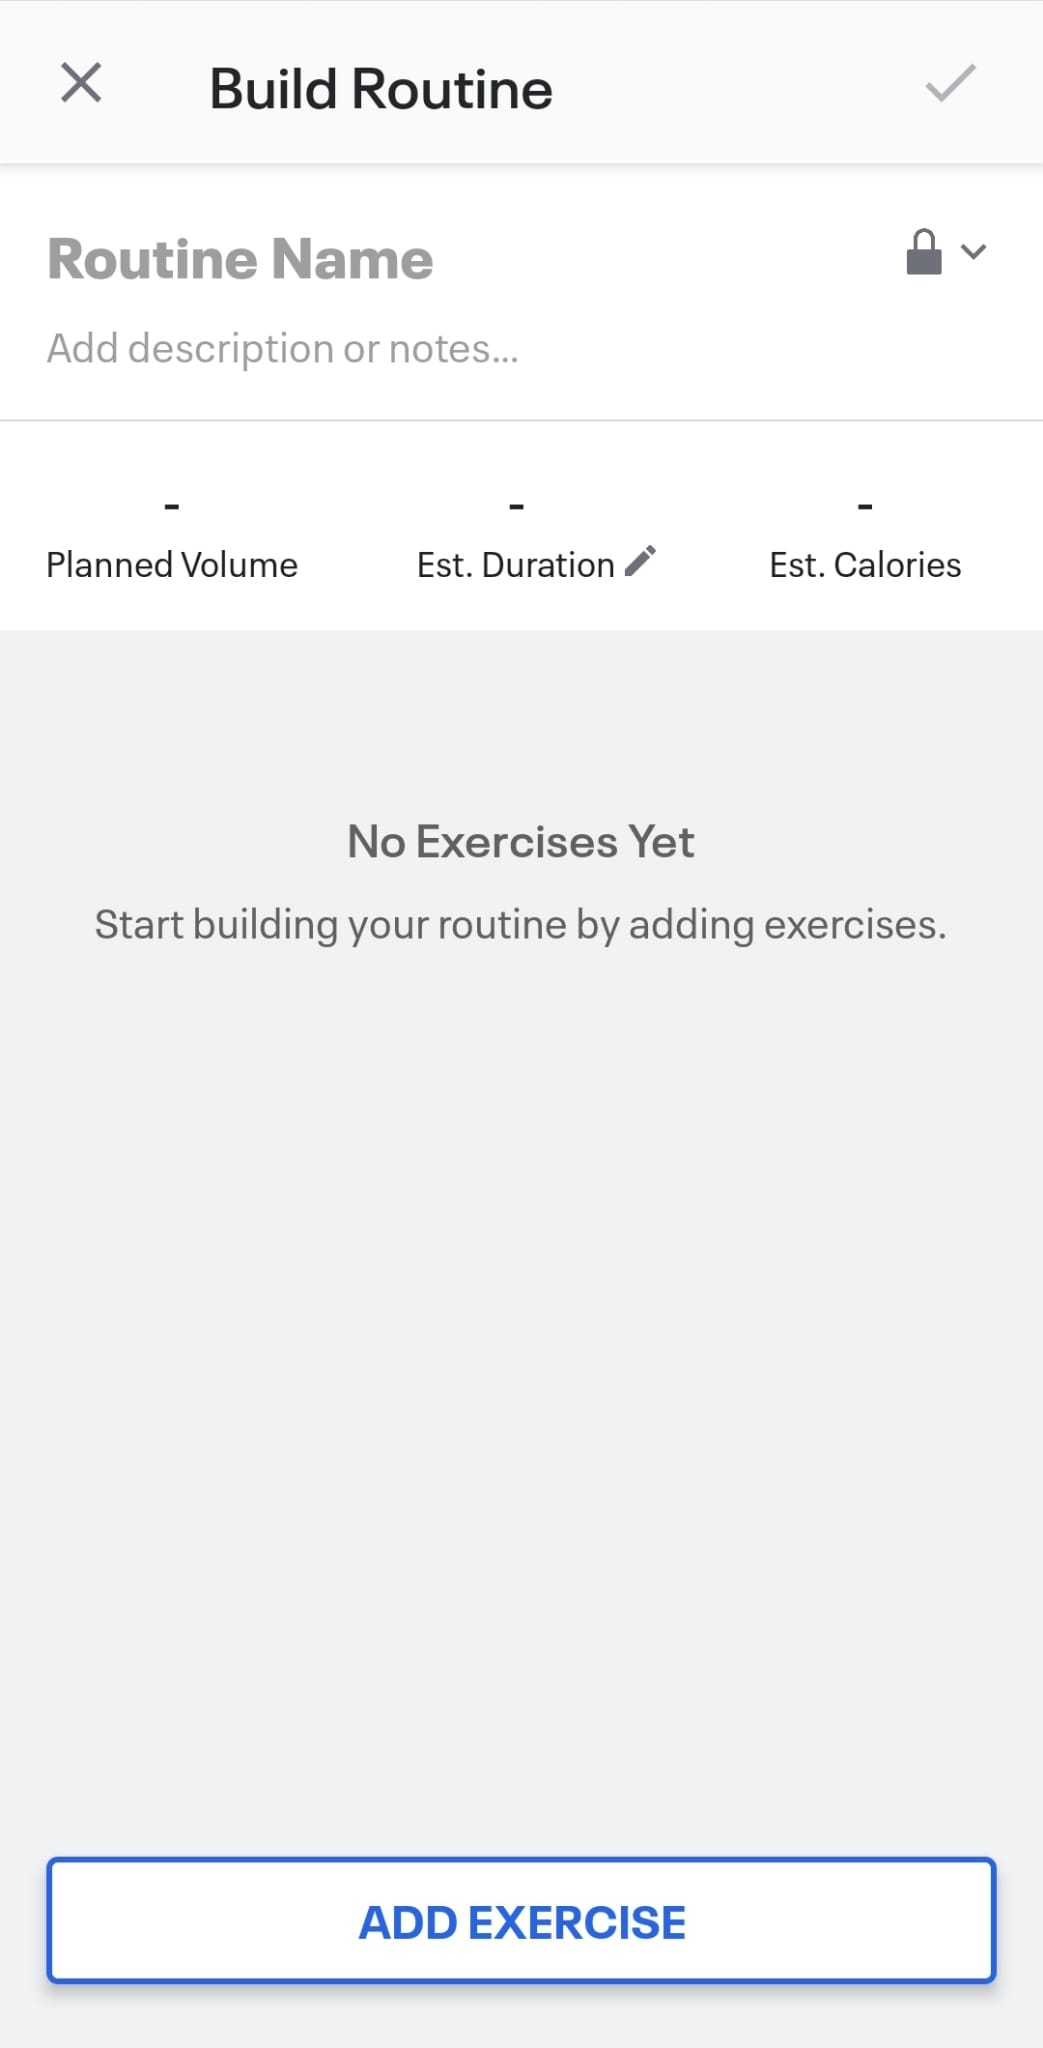
\includegraphics[width=0.5\textwidth]{myfitnesspal/exercise-routines.jpeg}
        \label{fig:mfp-workouts}
    \end{minipage}%
    \begin{minipage}{0.5\textwidth}
        \centering
        \includegraphics[width=0.5\textwidth]{myfitnesspal/exercise-choice.jpeg}
        \label{fig:mfp-exercise-picker}
    \end{minipage}
    \captionof{figure}{The custom workout routines in MFP}
    \label{fig:mfp-screens}
\end{figure}
\textbf{Features/Functionality}
\label{research-breakdown:mfp-features}
\par
MyFitnessPal includes all of the following features:
\begin{multicols}{2}
	\setlist{nolistsep}
	\begin{itemize}[noitemsep]
		\item Estimate calories burned given a set of exercises/a routine.
		\item Track food intake via barcode scan or recipe input.
		\item Track water.
		\item Workout plans provided by MFP.
		\item Track weight.
		      \columnbreak
		\item Create custom workout plans from existing exercises.
		      \setlist{nolistsep}
		      \begin{itemize}[noitemsep]
			      \item Exercises don't include video/images and no ability to add custom exercises.
			      \item These can be shared publically to dashboard.
		      \end{itemize}
		\item Count steps (using compatible devices).
		\item Add friends and send/receive messages.
		\item Community tab (requires separate signup).
		\item Export progress as CSV.
		\item Meal and weight tracking reminders (via push notifications).
		\item Set workout/week, minutes/workout and ``calories burned'' goals.
		\item Discover recipes/meal plans via community and MFP suggestions.
	\end{itemize}
\end{multicols}
\textbf{Technology Stack}
\label{research-breakdown:mfp-stack}
\par
MyFitnessPal uses the following technologies according to Stackshare \cite{mfp-stack}:
\begin{itemize}
	\item React (a JavaScript framework for creating cross-platform applications)
	\item Cloudflare (for web infrastructure)
	\item NginX (for server side use)
	\item Vanilla JavaScript and CSS + libraries (jQuery, Bootstrap)
\end{itemize}
Various other technologies are being used on the server-side but for \textit{the project}
we are primarily concerned with the technology used for the application
as opposed to the backend infrastructure.


\subsection{Fitbit}
Fitbit is the app that accompanies many of the Fitbit brands'
hardware products, their first movers advantage was likely
a large contributor towards their large market share (in 2018)\footnote{Q3 2020 wearables market share = 2.6\%\cite{fitbit-market-share}}
in the application space.
The functionality of their hardware products (which had been the standard for
fitness tracking wearables)
is enhanced through use of the app. The research will consider the application alone and disregard
any wearable-specific functionality.
\pagebreak
\begin{figure}[H]
    \begin{minipage}{0.5\textwidth}
        \centering
        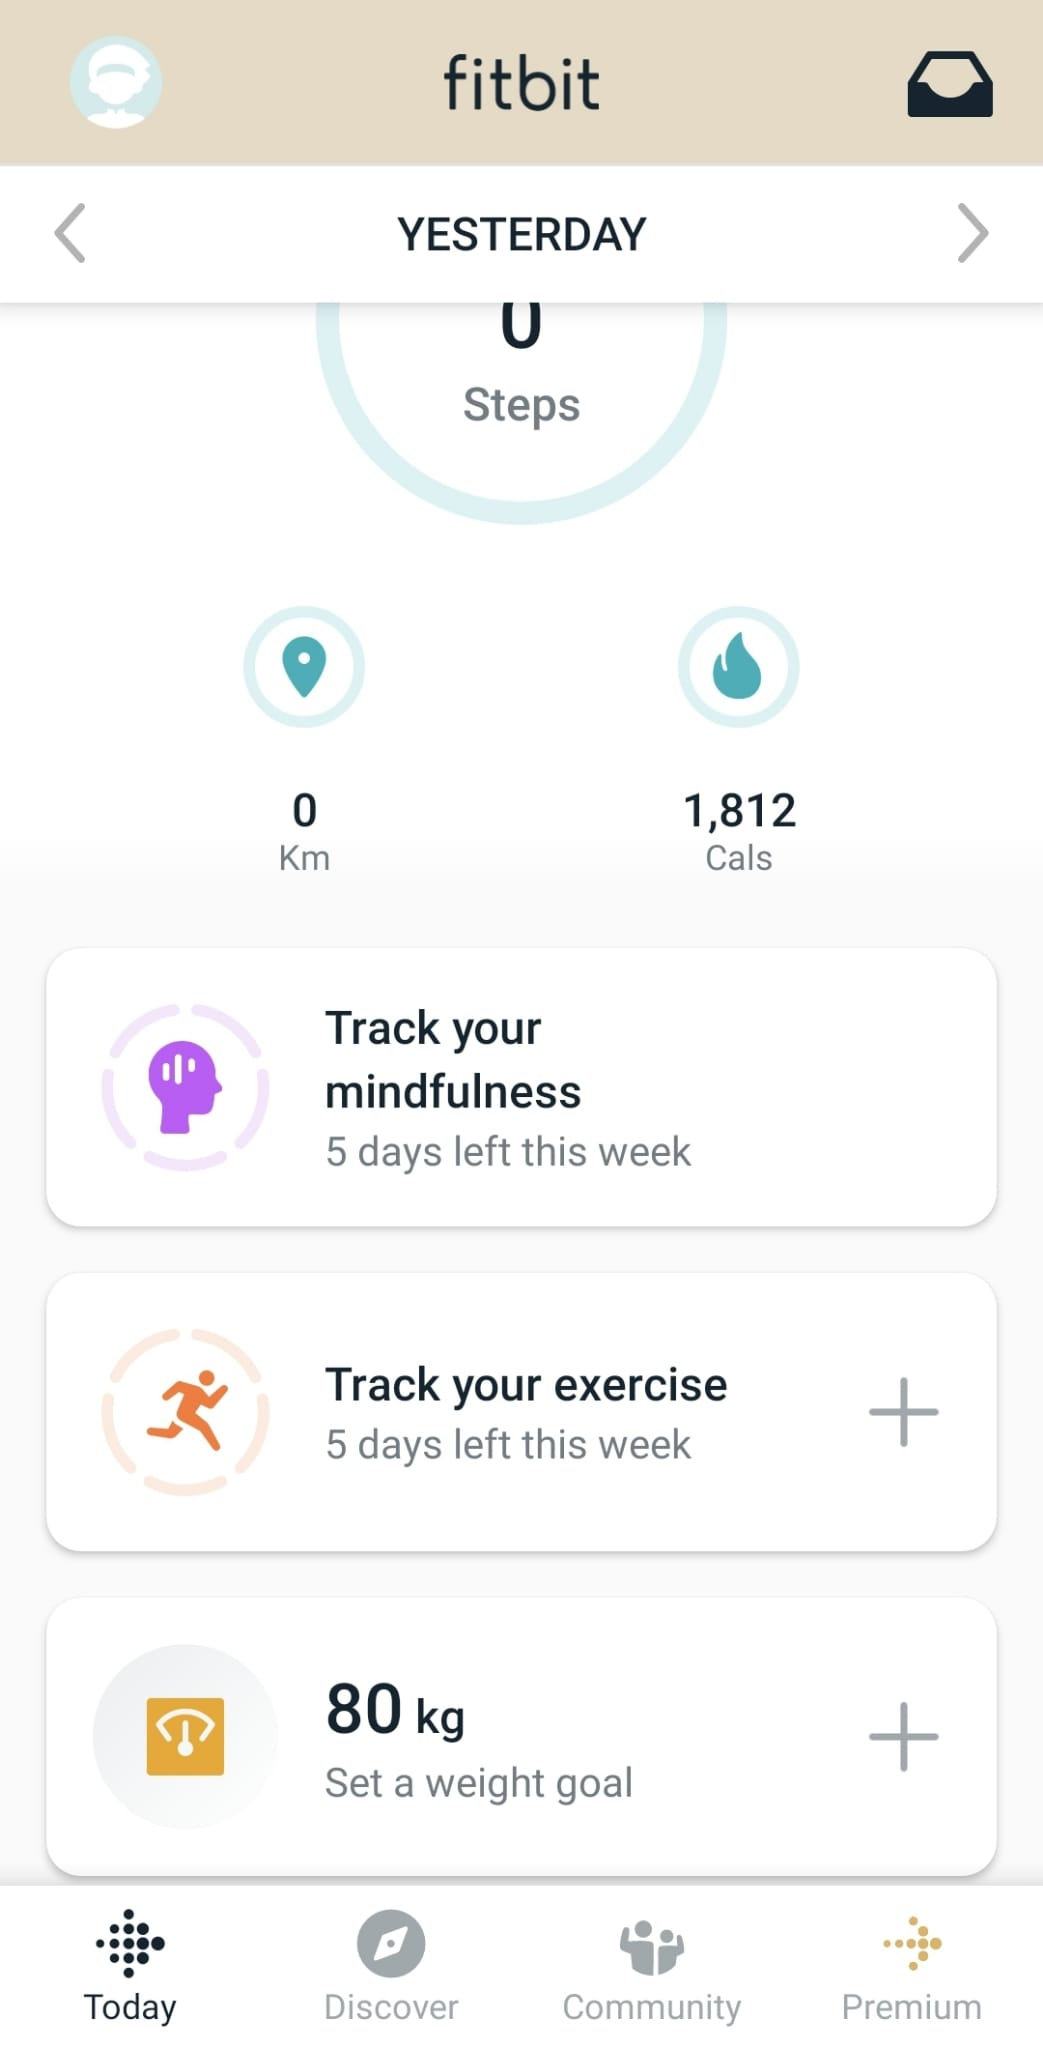
\includegraphics[width=0.5\textwidth]{fitbit/dashboard.jpeg}
        \caption{Dashboard}
        \label{fig:fitbit-home}
    \end{minipage}%
    \begin{minipage}{0.5\textwidth}
        \centering
        
\includegraphics[width=0.5\textwidth]{fitbit/food-tracker.jpeg}
        \caption{Food log screen \& features}
        \label{fig:fitbit-log}
    \end{minipage}
\end{figure}
\textbf{User Story}
\label{research-breakdown:fitbit-usr-story}
\par
``As a professional athlete I wake up, go through guided meditation on my Fitbit calendar before weighing myself (\cref{fig:fitbit-home}).
I then log my breakfast and eat (\cref{fig:fitbit-log}), followed by my commute to practice
and logging my sport and duration (\cref{fig:fitbit-exercise-log}).''

\begin{figure}[H]
	\centering
	\includegraphics[width=0.25\textwidth]{fitbit/exercise-choice.jpeg}
	\caption{Using exercise search \& log}
	\label{fig:fitbit-exercise-log}
\end{figure}
\pagebreak


\textbf{Features/Functionality}
\label{research-breakdown:fitbit-features}
\par
Fibit includes all of the following features:
\begin{multicols}{2}
	\setlist{nolistsep}
	\begin{itemize}[noitemsep]
		\item Guided meditation (w/ simple week-calendar scheduling).
		\item Guided video workout plans (w/ simple week-calendar scheduling).
		\item Guided programmes (for meeting targets in health, not just fitness).
		\item Challenges (1-10 people, gamifying targets).
		\item Water tracking.
		\item Food tracking.
		\item Track exercise (only by sport/activity, no custom option and no individual exercises/routines).
		\item Step counter.
		\item Community feed and groups.
		\item Add friends and send/receive messages.
	\end{itemize}
\end{multicols}
\textbf{Technology Stack}
\label{research-breakdown:fitbit-stack}
\par
Fitbit uses the following technologies according to Stackshare \cite{fitbit-stack}:
\begin{itemize}
	\item JavaScript(and Ember.js) for the front end.
	\item Fastly (for cloud content delivery)
	\item Redis (for middle layer and database caching)
	\item Node.js (for producing backend APIs)
	\item Java (and Spring) for the non-mobile applications
	\item MySQL (for the backend database(s))
\end{itemize}
Fitbit is cross-platform and multifunctional, thus there will be some technologies
not in use by the mobile app we are researching. It's unlikely Spring
is in use, but the use of JavaScript (w/ Node.js) for the front and backend is
common in current world of software. It's highly likely
the whole system is using a microservice architecture where components maybe used in several places.
\pagebreak

\subsection{Comparing MyFitnessPal and Fitbit}


\pagebreak
\subsection{TrueCoach}
TrueCoach provide a cross-platform system that includes a web application.
We'll be considering the mobile app provided for end users and making reference
to the functions available to administrators in the process. They provide a mobile app
for each of these use cases - ``\textbf{TrueCoach for Clients}'' and ``TrueCoach Connect'' for trainers.
\begin{figure}[H]
	\centering
	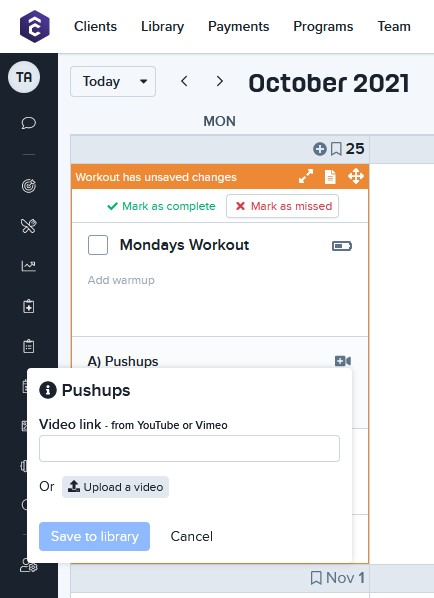
\includegraphics[width=0.3\linewidth]{truecoach/setting-client-workout.jpg}
	\caption{Trainer using web app to set clients workout(s).}
	\vspace*{-5mm}
	\label{fig:tc-trainer-set}
\end{figure}
\begin{figure}[H]
	\centering
	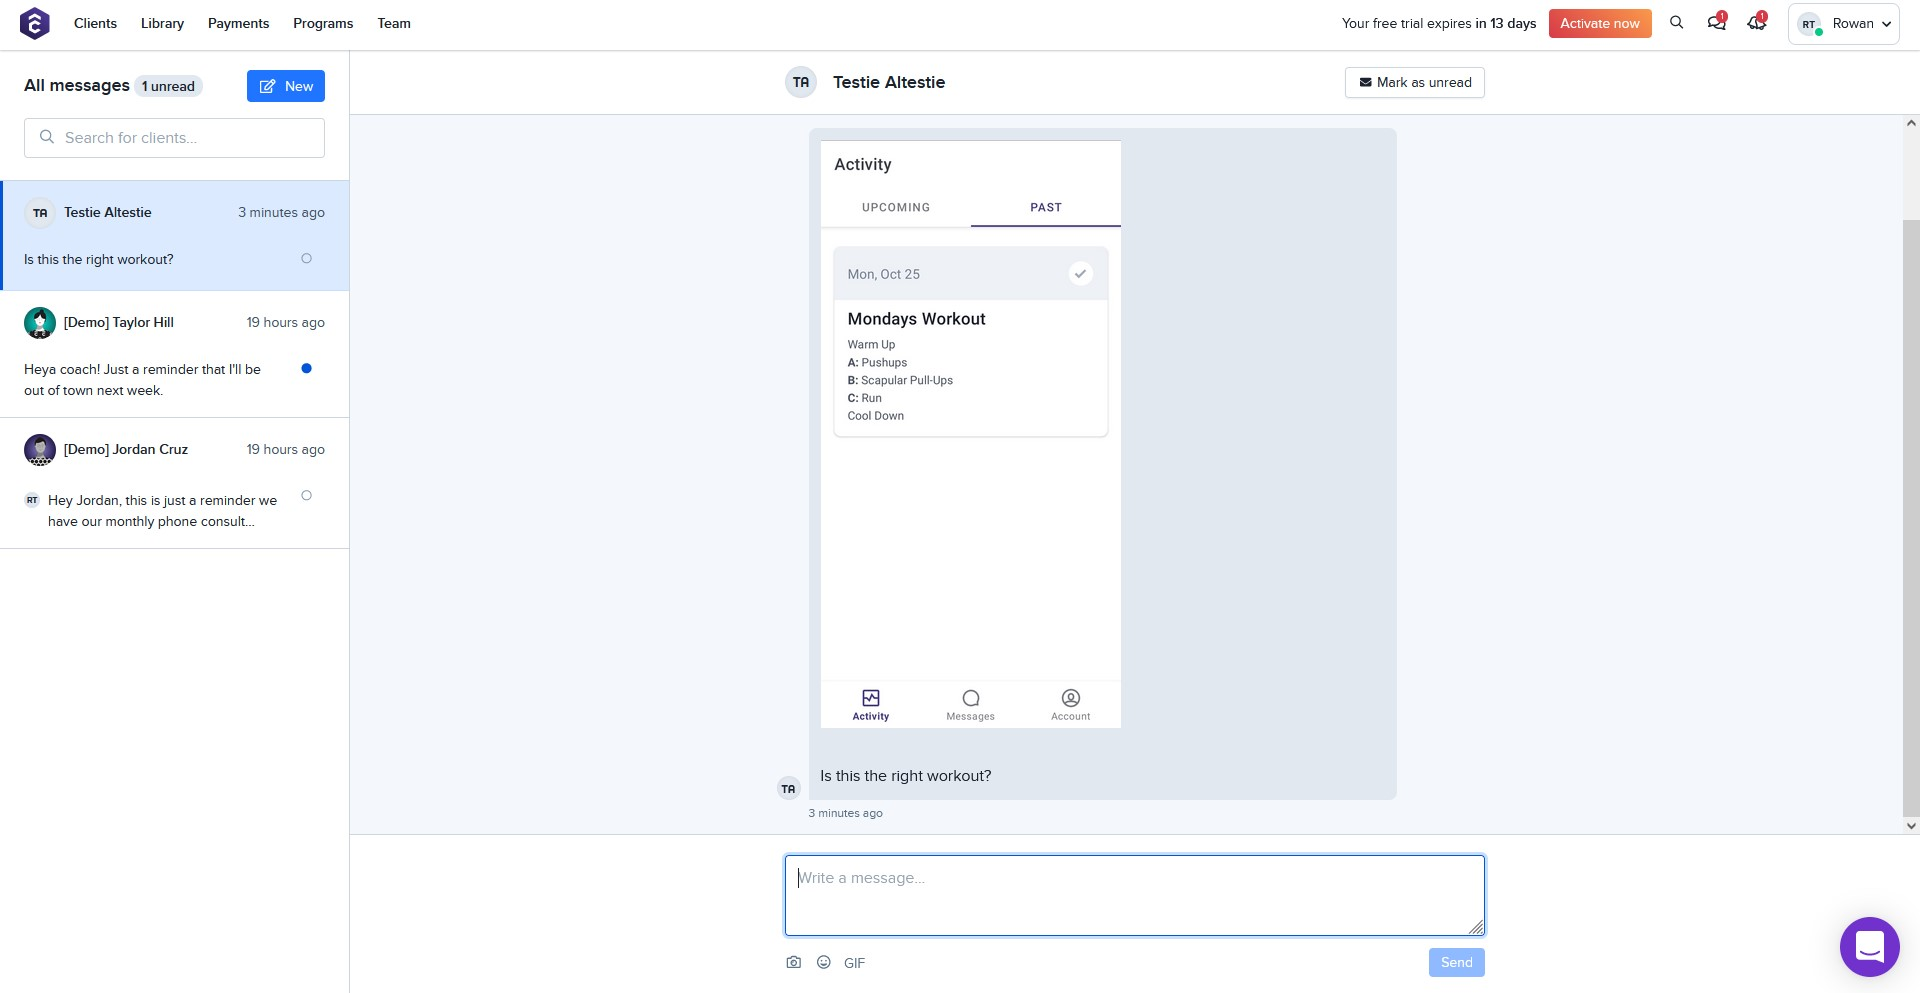
\includegraphics[width=1\linewidth]{truecoach/truecoach-web-chat.jpg}
	\caption{Trainer using web chat to manage clients.}
	\vspace*{-5mm}
	\label{fig:tc-trainer-chat}
\end{figure}
\textbf{User Story}
\label{research-breakdown:tc-usr-story}
\par
``As a new gym go-er, I work remotely with my trainer (\cref{fig:tc-trainer-chat}) to refine my training technique(s).
I follow instructional videos before marking my workouts as complete and monitoring 
my progress via goals \& challenges (\cref{fig:tc-workout}). For advice I can view
documents and progress photos in my settings page (\cref{fig:tc-settings}).''
\begin{figure}[H]
    \centering
    \begin{minipage}{0.4\textwidth}
        \centering
        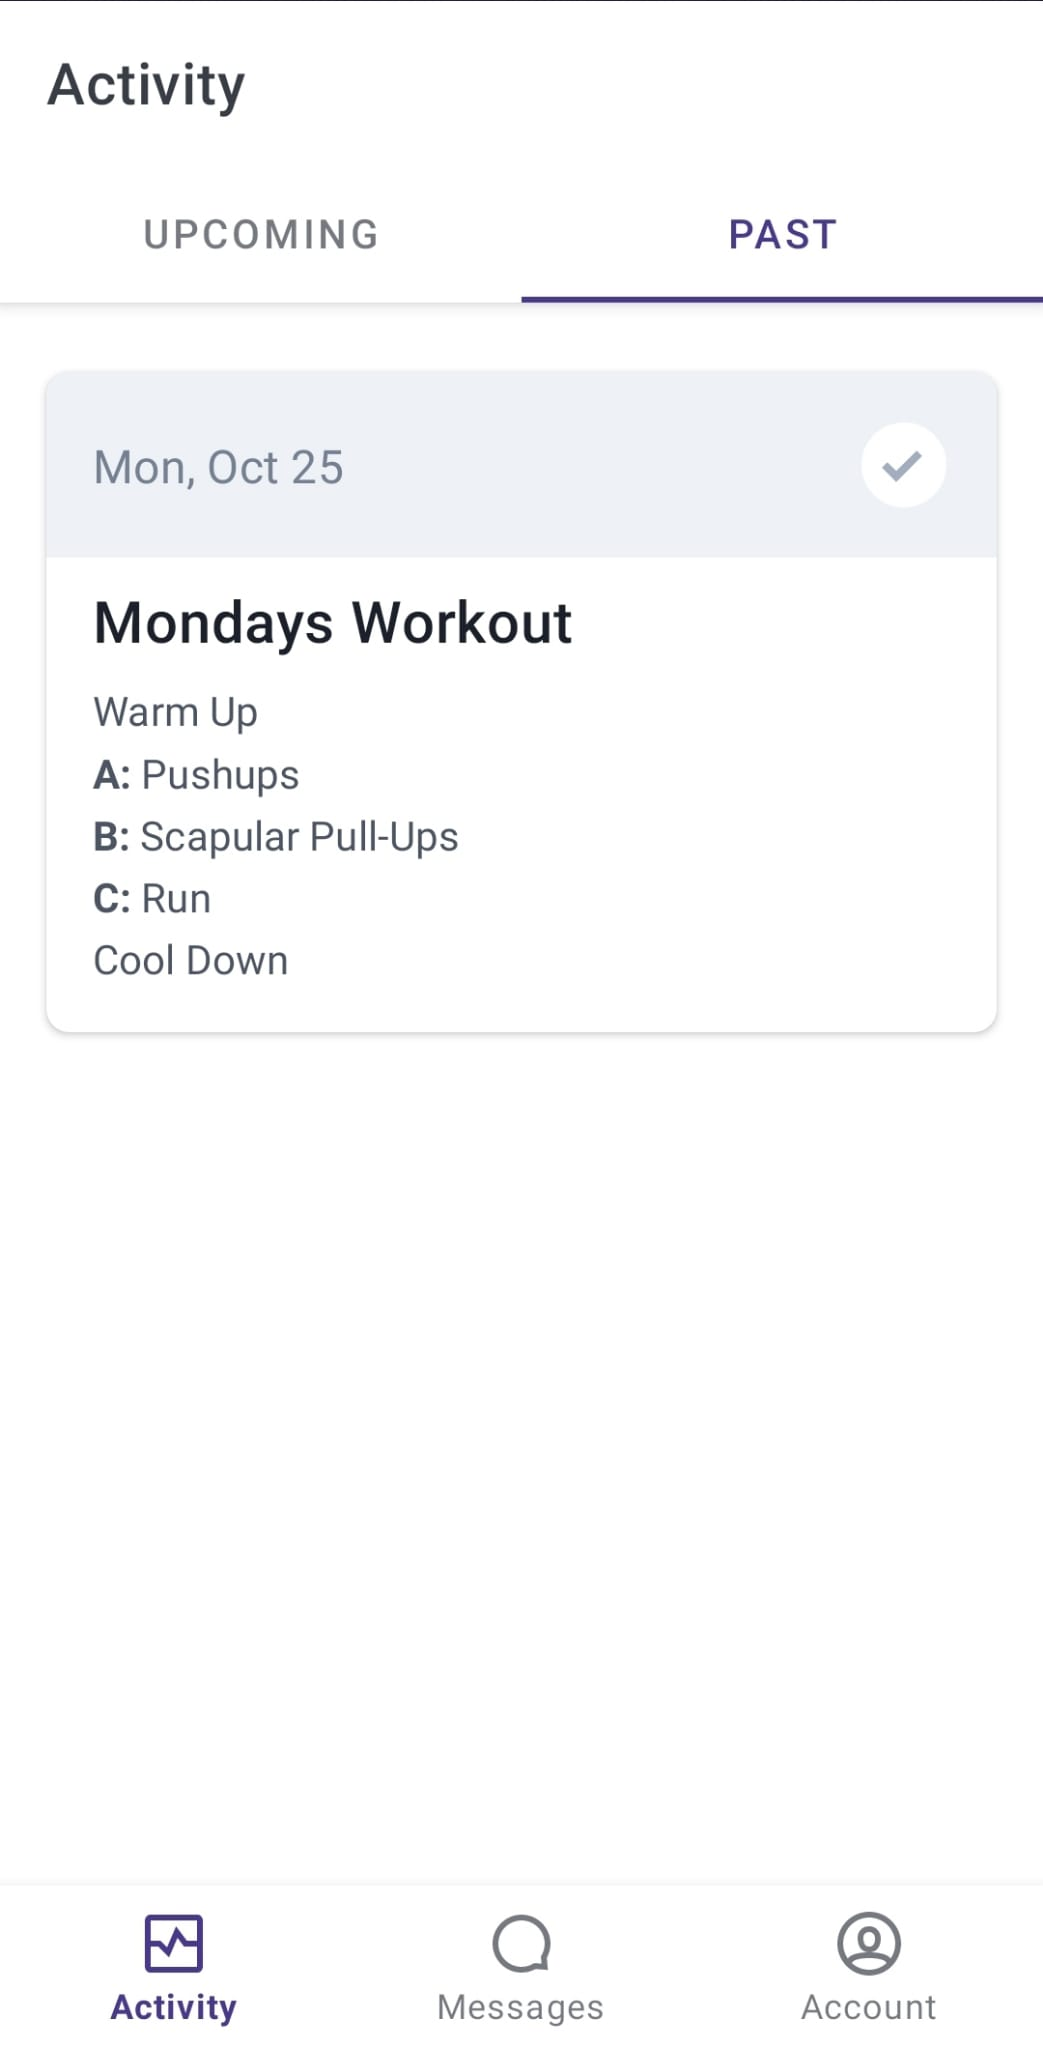
\includegraphics[width=0.5\linewidth]{truecoach/activity-page.jpeg}
        \caption{Viewing workouts (upcoming/past).}
        \label{fig:tc-activity}
    \end{minipage}\qquad
    \begin{minipage}{0.4\textwidth}
        \centering
        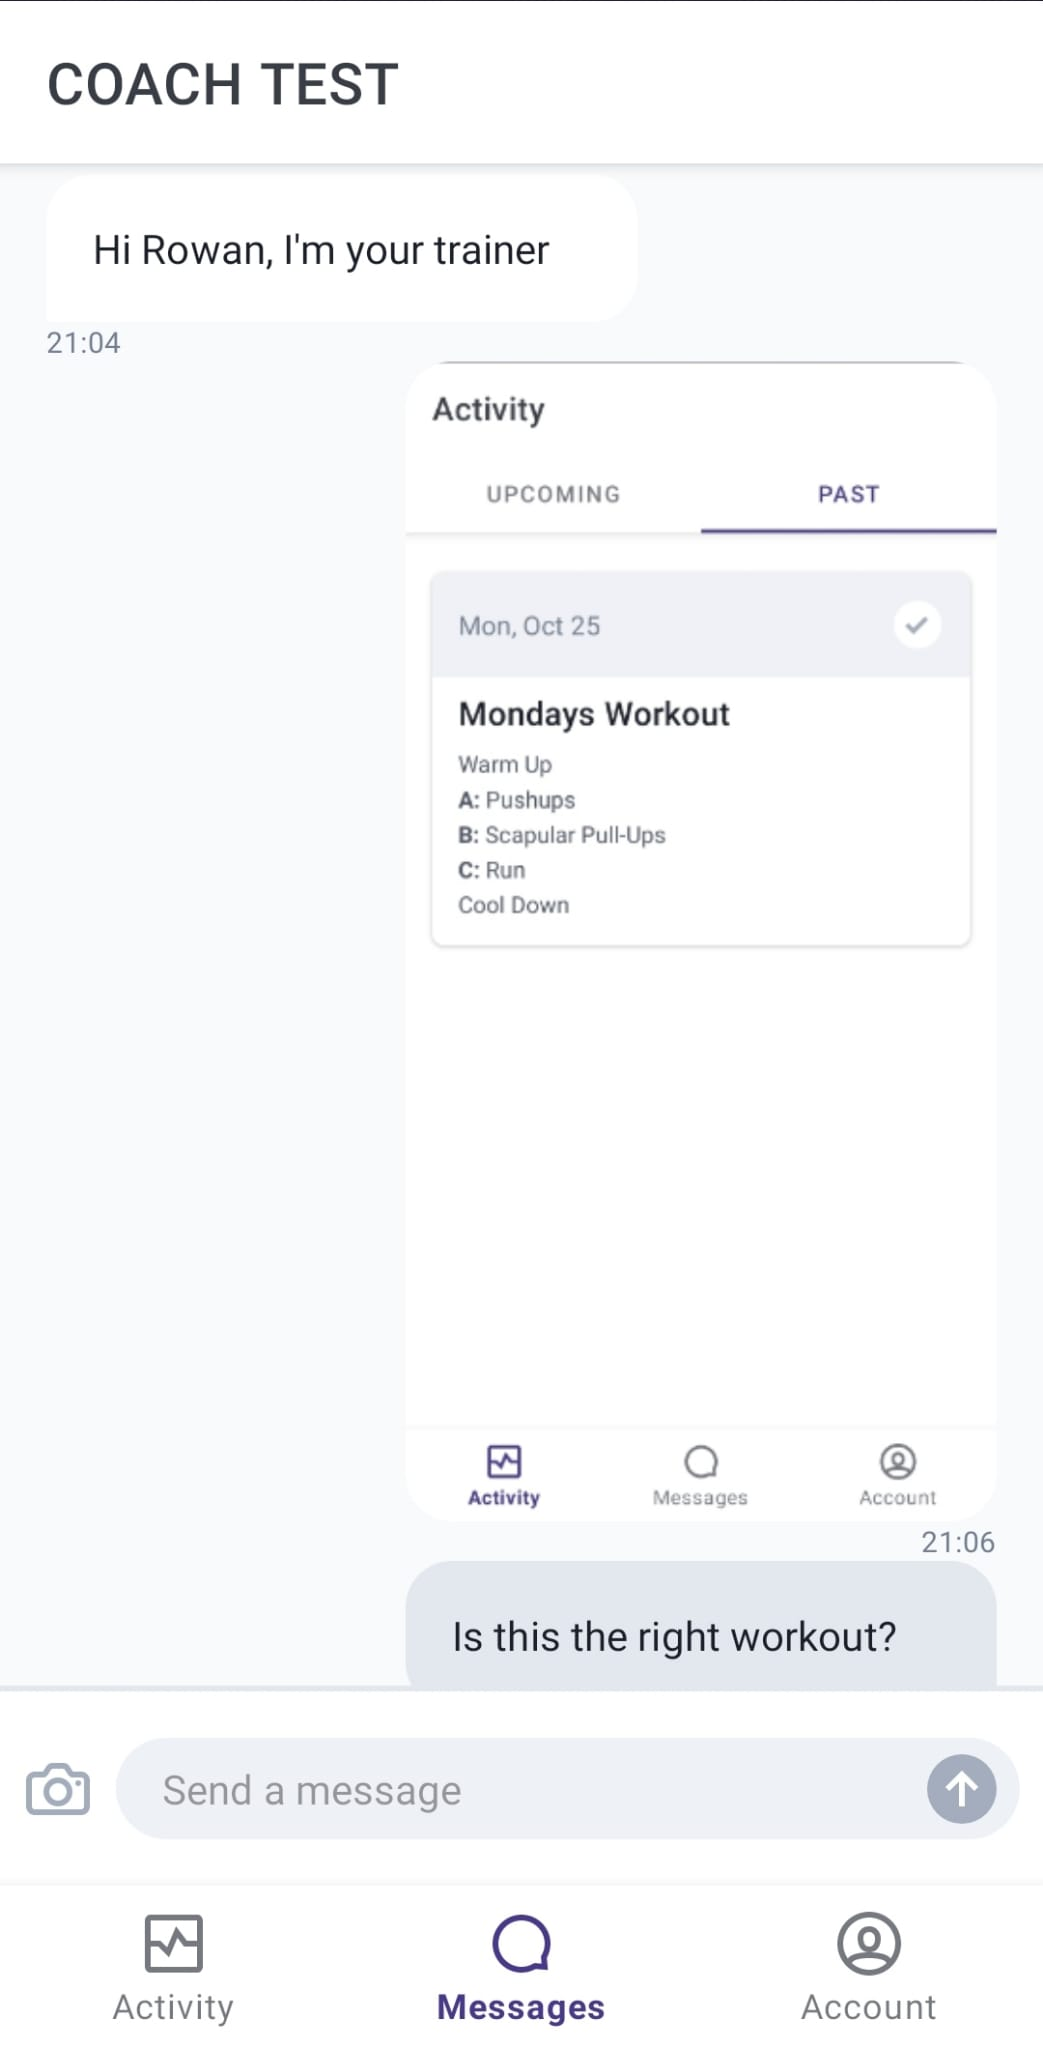
\includegraphics[width=0.5\linewidth]{truecoach/trainer-chat.jpeg}
        \caption{Instant messaging with a trainer.}
        \label{fig:tc-user-chat}
    \end{minipage}%
\end{figure}
\begin{figure}[H]
    \centering
    \begin{minipage}{0.4\textwidth}
        \centering
        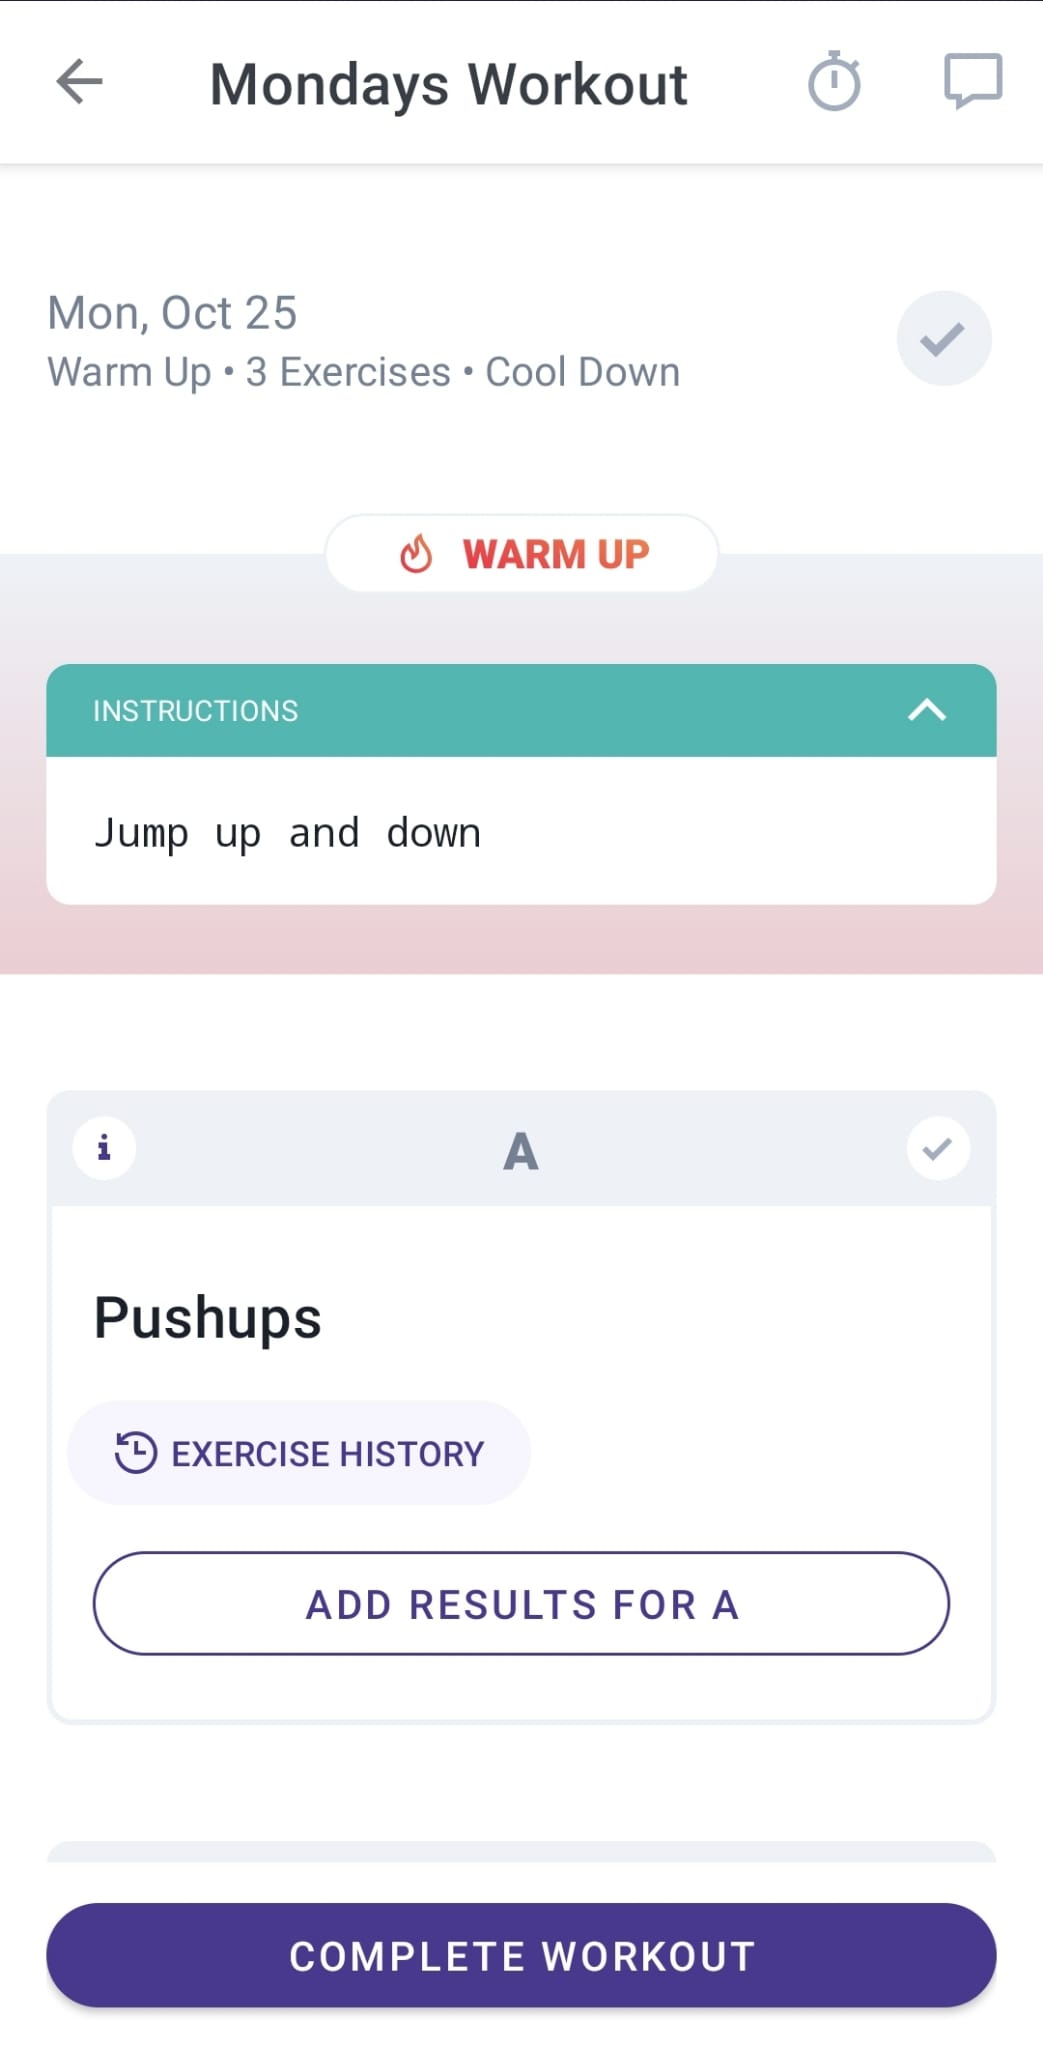
\includegraphics[width=0.5\linewidth]{truecoach/workout-logging.jpeg}
        \caption{Logging a workout.}
        \label{fig:tc-workout}
    \end{minipage}\qquad
    \begin{minipage}{0.4\textwidth}
        \centering
        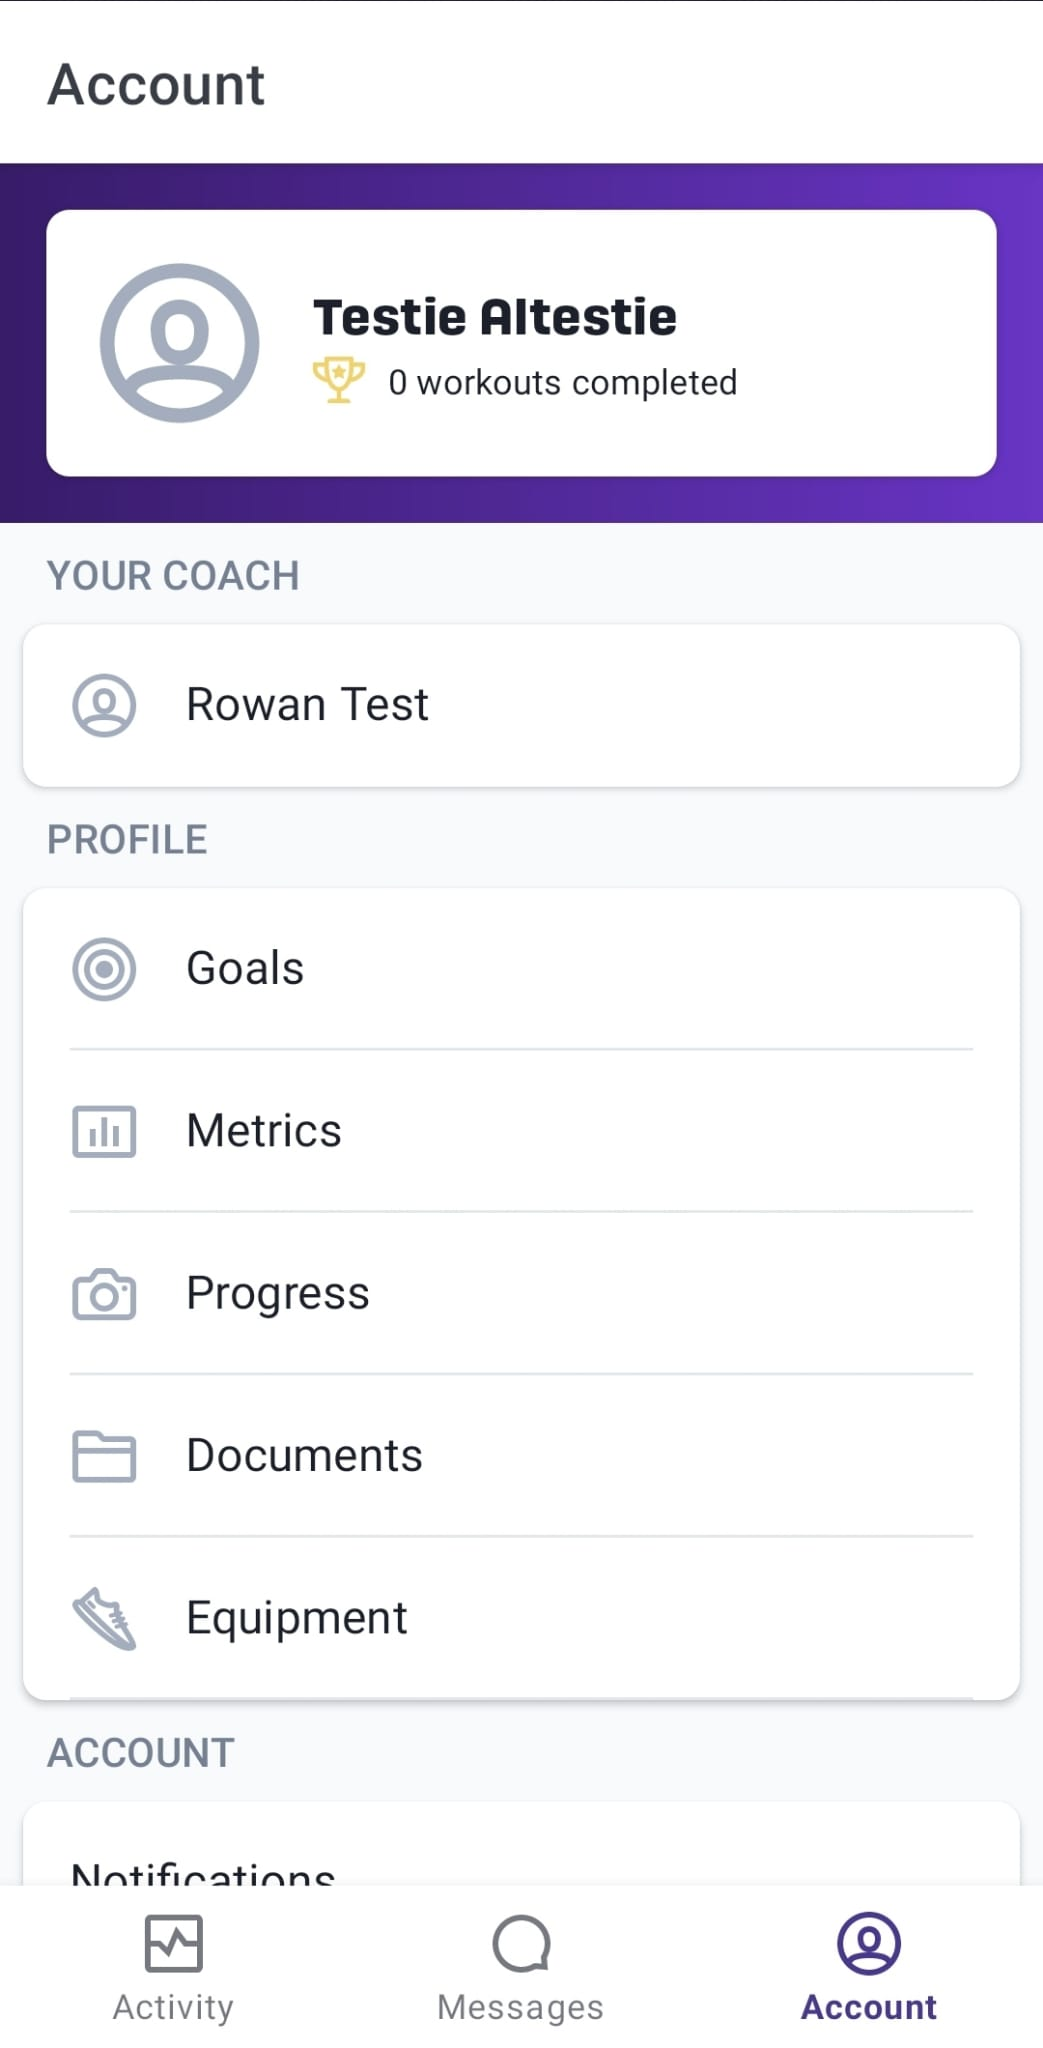
\includegraphics[width=0.5\linewidth]{truecoach/settings.jpeg}
        \caption{Viewing settings.}
        \label{fig:tc-settings}
    \end{minipage}%
\end{figure}
Above, ``Testie Altestie'' represents an end user and ``Rowan Test'' is the trainer. We can see
the functions available to the user are dependent on the workouts uploaded/scheduled
by the trainer using their interface (web application in this case).
\pagebreak

\textbf{Features/Functionality}
\label{research-breakdown:tc-features}
\par
\textbf{``TrueCoach for Clients''} includes all of the following features:
\begin{multicols}{2}
	\setlist{nolistsep}
	\begin{itemize}[noitemsep]
		\item Track coach's release of phased training (upcoming/past workouts).
		\item Log workouts (w/ notes).
		\item Timer \& stopwatch function for tracking timed exercises.
		\item Video breakdowns of exercises (w/ rich text instructions).
		\item Instant messaging w/ trainer (including multimedia uploads).
		\item Tracking of progress via trainer-set goals \& metrics.
		\item Progress and additional documents (outbound link to web app).
		\item Create account via invite link from trainer.
	\end{itemize}
\end{multicols}
\vspace*{-5mm}
TrueCoach covers a lot of needs for a user, and we can see in \cref{fig:tc-trainer-chat} 
the relevant tools for the trainer to facilitate these workouts. They are administrators of their
clients and they're the means by which a user gets login credentials. 
Trainers can upload relevant videos (\cref{fig:tc-trainer-set}) and documents, as well as provide metrics
to measure users progress.
\par
\textbf{Technology Stack}
\label{research-breakdown:tc-stack}
\par
Stackshare (as used for the previous apps) is not useful in this case, so the following conclusions have
been drawn following the decompilation of the TrueCoach APK \cite{apk-decompiler}.
\begin{itemize}
	\item Kotlin \& Java (for Android development)
	\item AWS Amplify (for backend deployment)
	\item Firebase (for push notifications)
\end{itemize}
After decompiling and opening the class files using \href{https://github.com/pxb1988/dex2jar}{dex2jar} and
\href{https://java-decompiler.github.io/}{JD-GUI}, I found that the application is not using a cross-platform
JavaScript framework as is standard in modern times. The app is using the recommended native language
of Kotlin\footnote{Learn more: \href{https://developer.android.com/kotlin}{android development documentation}} and Java for all data objects and frontend display. 
\pagebreak

\subsection{Exercise.com}
Exercise.com are the company providing the white-labelled solution behind \href{https://online.pjfperformance.net/users/sign_in/}{PJFPerformance}.
We'll be using the \textbf{PJFPerformance} app to analyse their application.
\begin{figure}[H]
    \centering
    \begin{minipage}{0.5\textwidth}
        \centering
        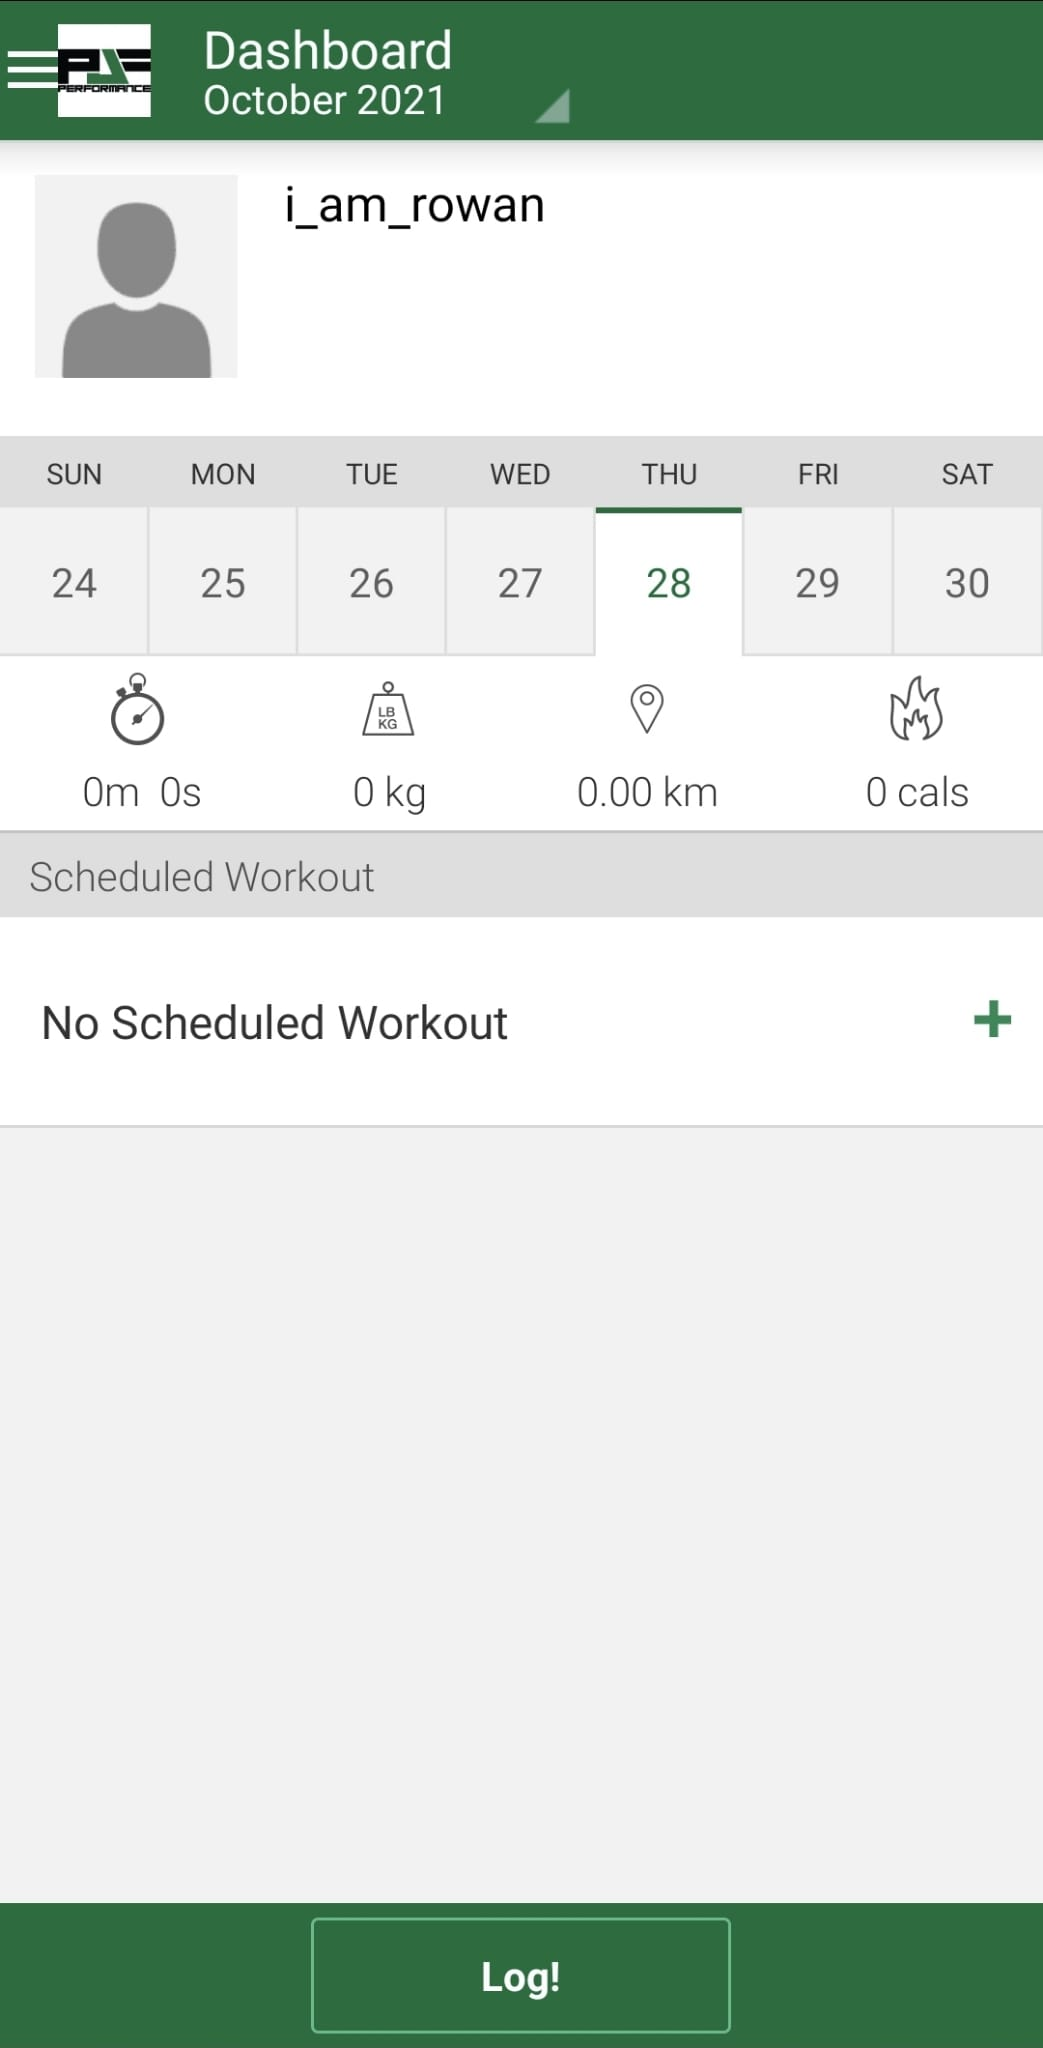
\includegraphics[width=0.5\textwidth]{pjf/pjf-dashboard.jpeg}
        \caption{Home dashboard}
        \label{fig:pjf-home}
    \end{minipage}%
    \begin{minipage}{0.5\textwidth}
        \centering
        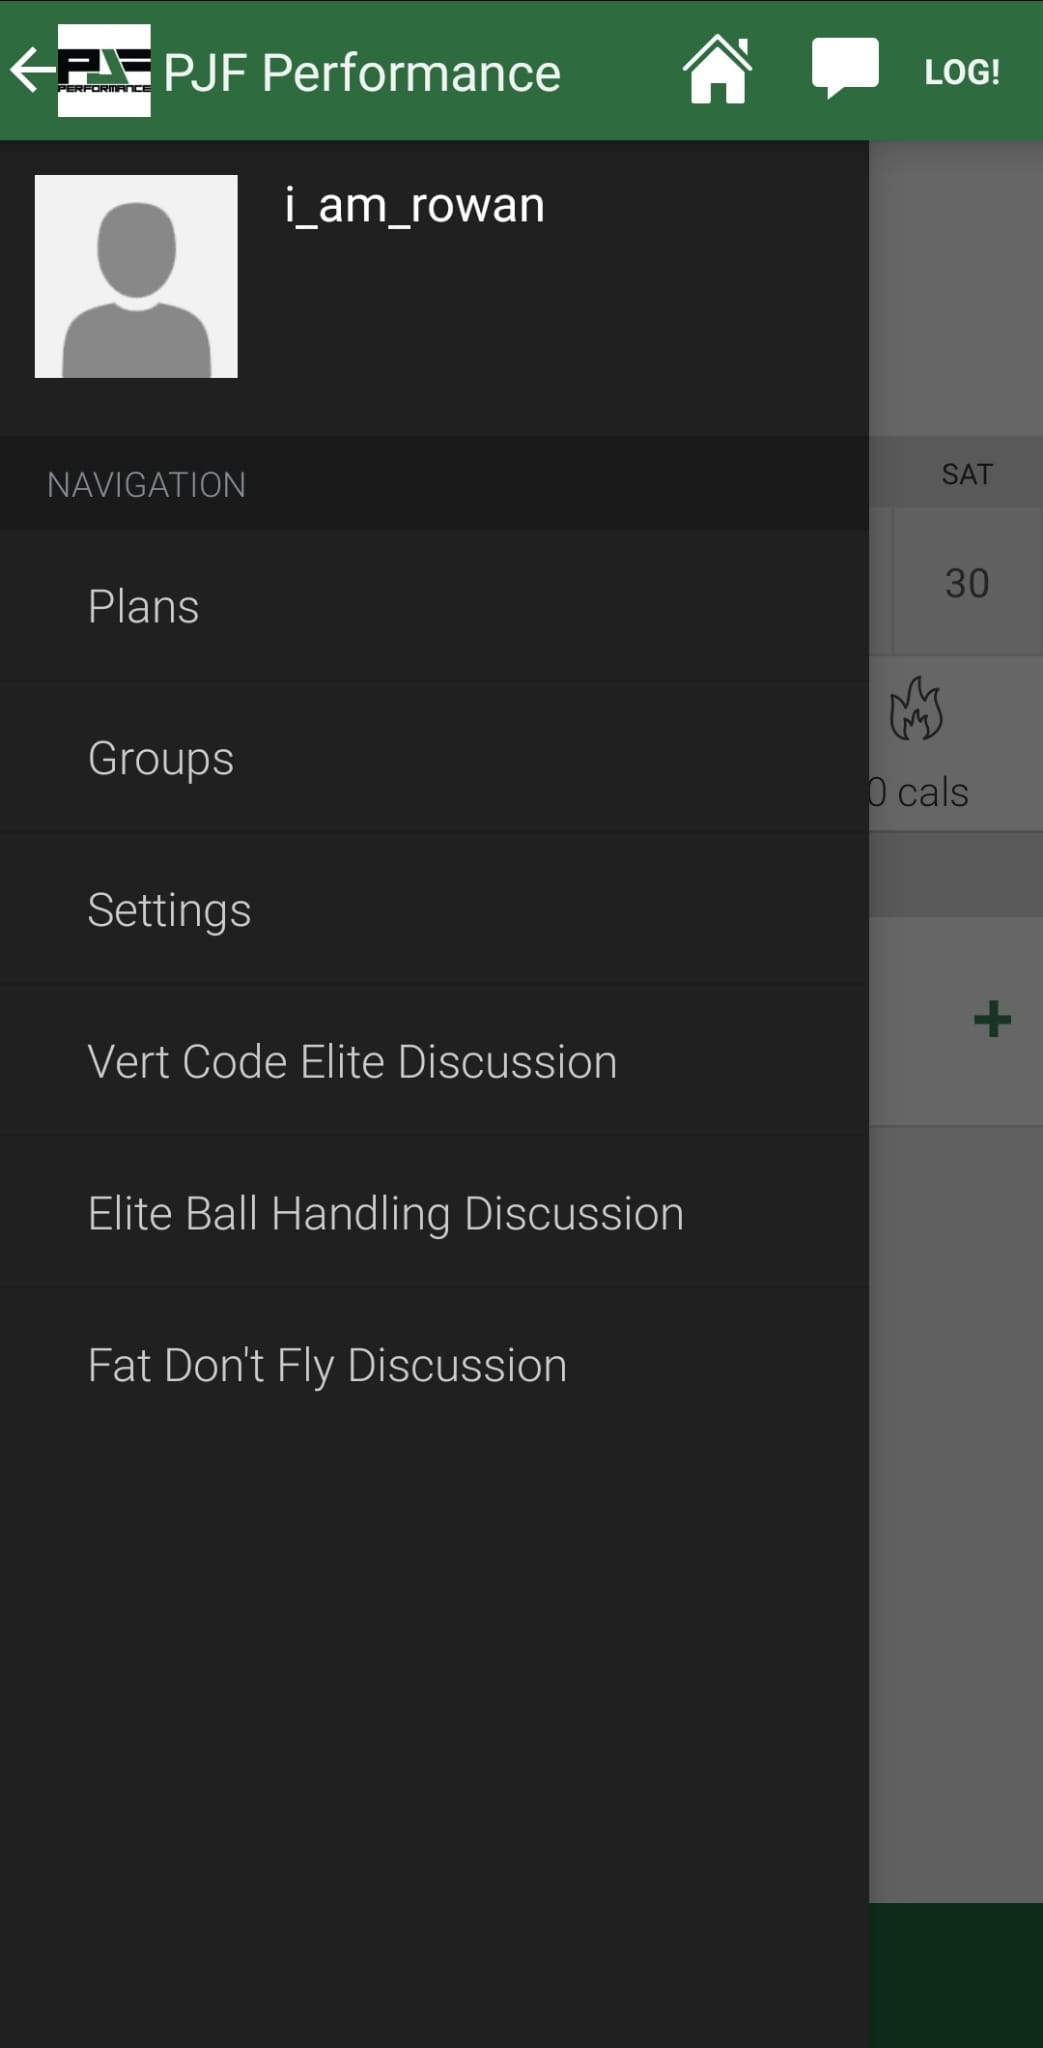
\includegraphics[width=0.5\textwidth]{pjf/pjf-menu.jpeg}
        \caption{Sidebar menu options}
        \label{fig:pjf-menu}
    \end{minipage}%
\end{figure}

\section{Existing vertical jump calculators}
\subsection{Maths behind calculating vertical jump using video}
\subsection{FitnessMeter - Test \& Measure}
\subsection{What's My Vertical?}
\subsection{My Jump 2}


\begin{itemize}
	\item \href{https://www.thehoopsgeek.com/measurement-app/#manual}{HoopsGeek App}
	\item \href{https://apps.apple.com/us/app/fitnessmeter-test-measure/id477488986}{Old ass iphone app}
	\item \href{https://apps.apple.com/gb/app/my-jump-2/id1148617550#?platform=iphone}{MyJump2 itunes}
	\item \href{https://www.youtube.com/watch?v=tIBiHDyev6w}{MyJump2 in use}
	\item \href{https://www.topendsports.com/testing/products/vertical-jump/video.htm}{Maths}
	\item \href{https://www.thehoopsgeek.com/the-physics-of-the-vertical-jump/}{Detailed maths courtesy of thehoopsgeek - legend}
\end{itemize}